\chapter{Results}

Proof of concept, as an example gesture or click traces were used as labels.
More general approaches can be used such as a description of the intent \cite{screen2words}, which needs another data set.

%\todo{overall goal is more than just interaction traces}
Make the algorithm as independent of the data as possible.
Find general rules to feed the data.
Applicable to other research fields, not just UI traces.
Use LSTM, so predict something unseen, in contrast to RICO or ERICA, which only categorize the current context

%Steps:
%- Data acquisition
%- Data cleaning / Preprocessing (Panadas)
%- Split into Training Data, Validation data, and Test data (cannot adapt the model after using the test data)
%- Train the model with the train data
%- Evaluate the model with the test data, then can adapt the model by the developer
%- Last deploy the model to production

\section{Datasets}

- Problem with sequential data sets

\subsection{Rico}

\begin{itemize}
  \item Too less frames.
  \item No transition between apps.
\end{itemize}

\section{Preprocessing Android UI tree data}
\subsection{Filtering privacy invasive details}

- rico doesn't use logins or any privat data
- gestures can tell more about the user
-


\subsection{Normalization, Feature selection}

Dealing with variable length data tf.io.VarLenFeature()

\section{Model}

%- Screen2Words

LSTM 4 dimensional
% https://stackoverflow.com/questions/54743549/is-it-possible-to-making-lstm-model-with-4-dimension-shape-of-data

Limitations to only 3 dimensions, needs flattening

Sample dimension (X -> y)
Time (Step) Dimension
Feature Dimension
Data, Quantity dimension, such as Image dimensions, or multiple nodes

TimeDistributedLayer
% https://stackoverflow.com/a/61588937/5164462
% https://stackoverflow.com/questions/53107126/what-are-the-uses-of-timedistributed-wrapper-for-lstm-or-any-other-layers


Multiple approaches

\todo{create graphic for each approach}

AutoEncoder:

\begin{itemize}
  \item Encoder -> Decoder -> LSTM -> Decoder
  \item Encoder -> LSTM -> Decoder
  \item LSTM -> Encoder -> Decoder (AutoEncoder)
\end{itemize}

Decoder can either only decode to x and y or to whole UI tree.

\section{Evaluation}

\begin{figure}[htbp!]
  \centering
  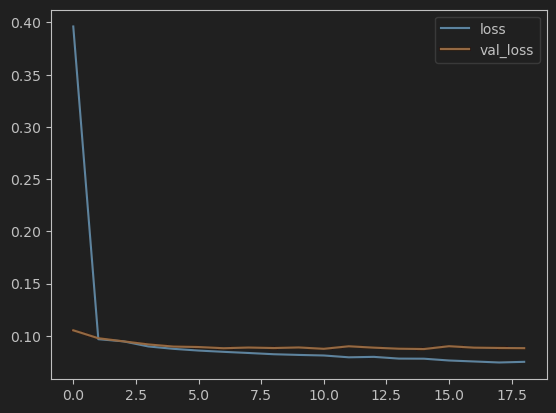
\includegraphics[width=\textwidth]{graphics/model_history_loss}
  \caption{Model loss vs validation loss}
  \label{fig:model_history_loss}
\end{figure}

\subsection{Mean Squared Error}

\section{Limitations}

Dataset
Dataset is not through different apps, only in one app.
Dataset is not detailed enough in the time steps, or not containing all data
Dataset is not long enough
Dataset has no paid apps or apps with login, which most services require
Dataset has wrong data see \cite{clay}

Preprocessing
Need more time to validate what are the core parameters to predict the next user intent


Model needs more investigation on what data is needed
How many neurons are required to achieve this
Play around with different layers, also Convolutional and pretrained embeddings

